\subsection{Future Software Research}

Currently, the number of wires that our neural network outputs is constant. However, the complexity of the functions that the wire-fitting function has to model varies from task to task. To add to the portability of Fido, we plan on implementing a method of dynamically changing the number of wires that the neural network outputs. Such a method would gage the variance and bias that the interpolator is experiencing. Variance is the deviation of a function from its mean. Bias is the error that results from under fitting. The wire-fitting function's variance could be measured in a range of actions. Bias could be measured as the moving average of the wire-fitted interpolator function's error at predicting Q-values, or the moving average of the distance that the wire-fitting function's wires have to move during gradient descent. Our proposed method would look to reduce $bias^2 + variance$ by increasing the number of wires if there is high bias squared and decreasing the number of wires if there is high variance. Each time a wire is removed or added to create a new set of wires, this set of wires will be changed to best model the wire-fitting function formed by the past set of wires.

The topology of our feed-forward neural networks is static throughout Fido's lifetime. To increase the generality of Fido, we would like to research ways to evolve the topology of Fido's neural network as performs action and receives reward. This may mean measuring variance and bias values and determining the direction of $bias^2 + variance$ as outlined above, but may also take the form of an existing variation of back propagation, of which there are many.

\subsection{Hardware Implementation}

\begin{figure}[ht]
	\centering
	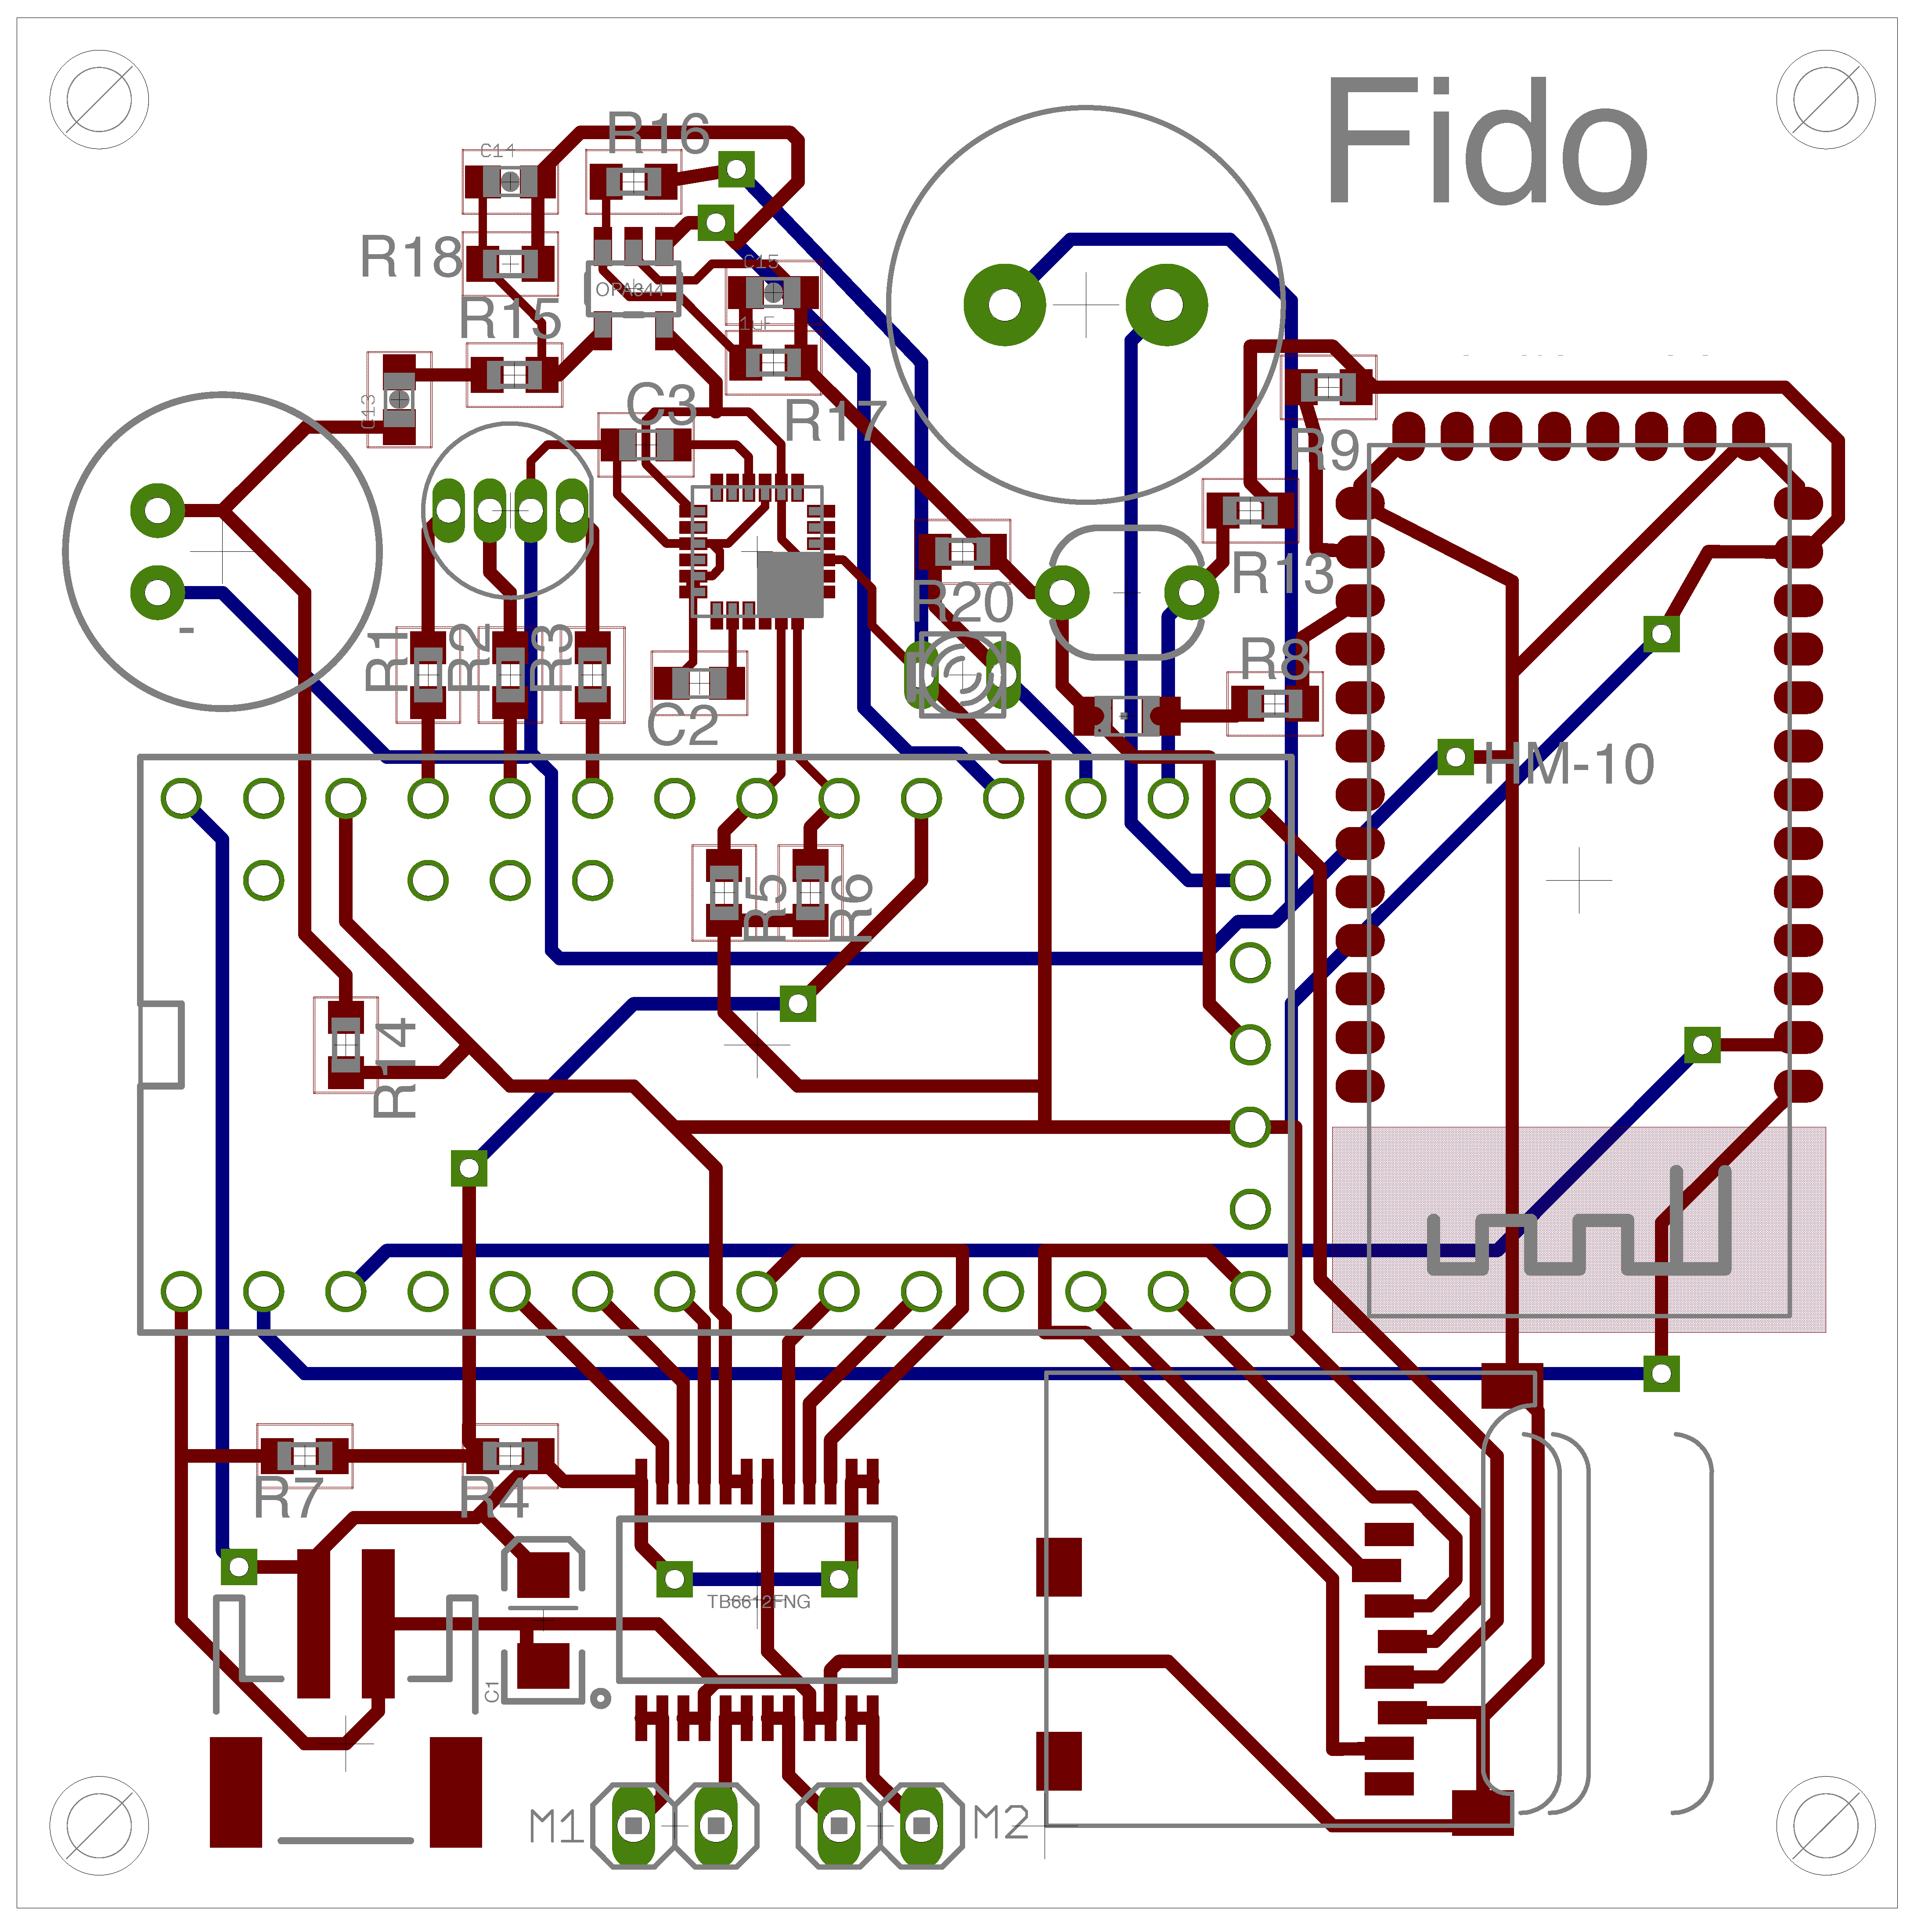
\includegraphics[height=7cm]{Figures/boardLayout.png}
	\caption{Fido PCB Layout}
\end{figure}

A schematic and printed circuit board have been designed for Fido's hardware implementation, and are the next step in testing and improving the Fido control system.  The PCB was modeled after the simulator reference design, and as such contains dual motor control, a photo-resistor for visible light, a photo-transistor for infrared light, etc.  The board (designed in CadSoft Eagle) operates off of the Teensy 3.1 microcontroller development platform, which combines a 96Mhz ARM Cortex M4 microcontroller and a USB bootloader for easy debugging.  The software base is in the process of being ported to the avr-gcc compiler toolchain for microcontrollers, a feat only possible through a small code footprint and low reliance on C++ Standard Library functionality.